	\documentclass[9pt,twocolumn,twoside]{osajnl}


%\usepackage{csquotes}
\usepackage{tikz}
%\usepackage{graphicx}


\journal{josaa} % Choose journal (ao, josaa, josab, ol)

\setboolean{shortarticle}{false} % true = letter, false = research article


\title{On the analogy between curved space-time and non-impedance-matched anisotropic media }

\author[1]{S. A. Mousavi}
\author[2*]{R. Roknizadeh}
\author[3,4]{SH. Dehdashti}
\author[5]{S. Sahebdivan}

\affil[1]{Department of Physics, Faculty of Science, University of Isfahan, Hezar Jerib, Isfahan, 81746-73441, Iran}
\affil[2]{ Department of Physics, Quantum Optics Group, Faculty of Science, University of Isfahan, Hezar Jerib, 81746-73441 Isfahan, Iran}
\affil[3]{State Key Laboratory of Modern Optical Instrumentations, Zhejiang University, Hangzhou 310027, China}
\affil[4]{The Electromagnetic Academy at Zhejiang University, Zhejiang University, Hangzhou 310027, China}
\affil[5]{Quantum Optics, Quantum Nanophysics and Quantum Information, Faculty of Physics, University of Vienna, Boltzmanngasse 5, 1090 Wien}
\affil[*]{Corresponding author: r.roknizadeh@gmail.com}

\dates{Compiled \today}

\ociscodes{(160.1190)  Anisotropic optical materials,(160.3918) Metamaterials, (260.2110)   Electromagnetic optics }

\doi{\url{http://dx.doi.org/10.1364/ao.XX.XXXXXX}}

\begin{abstract}


An electromagnetic medium with gradient refractive index can resemble a geometrical analogy with an arbitrary curved space-time, only if it fulfils the condition of impedance-matching with vacuum \cite{leonhardt2006general}. 
In this paper, we study the properties of a non-magnetic medium with a varying optical axis that can resemble the features of an optical metric.
A medium with a varying optical axis is an engineered stratified slab of materials, consist of thin layers, in which the orientation of optical axis would slightly varies, whereas, the magnitude of refractive index remains constant in the whole medium. 
The inhomogeneity in such a medium is induced by the local anisotropy in each layer: Instead of spatial change in the refractive index, the propagation of light depends on the local optical axis.
We study the conditions that make the analogy between curved space-time and a medium with a varying optical axis. To obtain the effective metric we apply the theory of transfer matrixes for the linear systems.
Extension of  the transformation optics to the media with optical axis profile might ease some fabrication cumbersome of  gradient refractive index materials for particular frequencies. 

\end{abstract}



\setboolean{displaycopyright}{true}

\begin{document}
\maketitle
\thispagestyle{fancy}
\ifthenelse{\boolean{shortarticle}}{\abscontent}{}

\section{Introduction}





 %-----------------------------------------------------------------------------------------------------------
\begin{figure}[top]
	 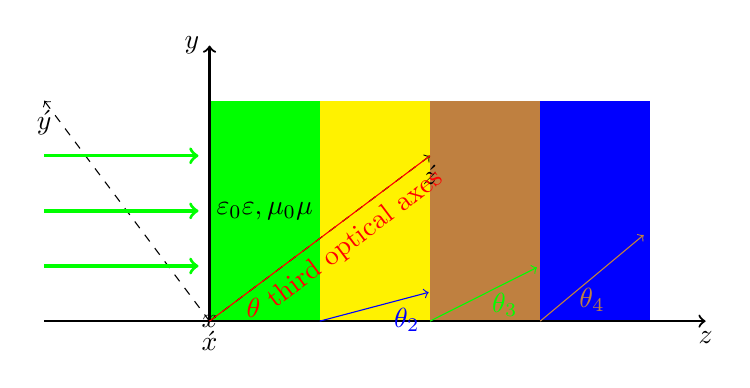
\begin{tikzpicture}[xscale=0.7, yscale=0.7]
		%\filldraw[fill=green!20!white, draw=green!40!black, very thick] (2,0) rectangle (4,4);
	    \fill[fill=green] (2,0) rectangle (4,4)node [pos=0.5]{$\varepsilon_0 \boldsymbol \varepsilon, \mu_0 \boldsymbol\mu $};
	   \fill[fill=yellow] (4,0) rectangle (6,4);
		   \fill[fill=brown] (6,0) rectangle (8,4);
			\fill[fill=blue!] (8,0) rectangle (10,4);
	%----------------------------------------------------------------------
			\draw [->,thick] (2,0) node{$x$} -- (2,5.0) node[left]{$y$} ;
		\draw [->,thick] (-1,0) -- (11,0) node [below]{$z$};
		\draw [-> ,dashed] (2,0)node [below]{$\acute{x}$} -- (6,3)  node [below]{$\acute{z}$};
	 \draw [-> ,dashed] (2,0) -- (-1,4) node [below]{$ \acute{y}$};
	%----------------------------------------------------------------------
	
	  \draw [red] (2,0) -- (6,3) node [pos=0.2, below]{$\theta$} node [pos=.6,below, rotate=37]{third optical axes} ;
		   \draw [->,blue] (0:4) -- (5:6)node [pos=0.8, below]{$\theta_2$};
		   \draw [->,green] (0:6) -- (7:8)node [pos=0.7, below]{$\theta_3$};
	 	   \draw [->,brown] (0:8) -- (9:10)node [pos=0.5, below]{$\theta_4$};
	
	%---------------------------------------------------------------------------------
		%	\draw (2,0) arc[radius = 1, start angle= 0, end angle= 37]
		    \draw [-> , green,very thick] (-1,1)  -- (1.8,1)  ;
		\draw [->,green,very thick] (-1,2)  -- (1.8,2) ;
			\draw [->,green,very thick] (-1,3)  -- (1.8,3)  ;
	    %    \draw [domain=-2:2, samples=50] plot (\x, {3x+1});
			
	\end{tikzpicture}
	\caption{Schematic of an anisotropic slab with $\boldsymbol{\varepsilon}$ and $\boldsymbol{\mu}$ as a tensor, light incidents from left and incident plane is $y-z$ plane; two principle axes of media  $z^{\prime}$ and $y^{\prime}$ do not lay on the $z$ and $y$ coordinate.}\label{figure1}
\end{figure}
%---------------------------------------------------------------------------------------------


Transformation optics works based on the diffeomorphic map between a virtual space and physical space. For technical simplification, usually physical space is an isotropic electromagnetic medium with a position dependent refractive index profile, while the optical axis of the medium is fixed. This simplification restricts the diffeomorphic maps to the family of quasi-conformal maps. 
However, inspired by optical axes grating in liquid crystals \cite{Sarkissian, NERSISYAN}, one can shows he transformation optics map between the virtual space and physical space is valid, if one varies the direction of optical axes instead of amplitude of refractive index \cite{liang2012transformation}.  In mathematical language the transformation map can extend from the family of angle preserving maps (quasi-conformal) to the family of area preserving maps \cite{}
Medium with a variable optical axes is an inhomogeneous anisotropic material that its inhomogeneity induces by the change in the direction of the optical axes. The direction of the optical axes in these media depends on the position.
These media can be realized by use of  liquid crystal with applying the external field or internally charged particles \cite{sluijter2010ray}.
Anisotropy and inhomogeneity in the medium is responsible for curving the light trajectories. In medium with a varying optical axis inhomogeneity is due to infinitesimal change of optical axis in each layer. In theory, each thin layer is an anisotropic optical  layer which the direction of optical axis is controllable. 
%In the anisotropic materials the propagation of light depends on the direction of optical axis, therefore, it is convenient to start  studying the propagation of light in a birefringent layer. 
%Inspired by the ray tracing methods, we derive the conformal metric for the normal incident on the slab of anisotropic birefringent material when the propagation of light is depend on the axis.
% As a result we show there is a non zero curvature for the associated to each metric of the light field in a birefringent  and impedance matched medium.

Anisotropic materials are accessible in nature and also much cheaper to design artificially. Crystals are the best-known materials that perform electrical anisotropy based on their particular crystal structure and the symmetry of their space group. Many plastics also are anisotropic, because their molecules are 'frozen' in a stretched conformation when the plastic is molded or extruded \cite{PEN}. 

Combination of many homogenous anisotropic layers, with infinitesimal variation  in the direction of optical axis, results in an inhomogeneous medium with optical axes profile.  In principle such medium can be a linear optical system. By the method of  the transfer matrix introduced by \cite{},  we show that a medium with the variable optical axes can consider as a curved space for light rays. Such materials show the capacity for being used in transformation optics designs when impedance-matched materials are costly. More elaborated theory of transformation optics with variable optical axes profile would appear shortly in the further publications.

The organisation of the paper is as follows: 
In section 2 we briefly introduce our material and methods used in this research.
In section 3, we explain a technique, eigenvalue wave equation method,  to solve the Maxwell equations in each layer of anisotropic medium. In section 4 we review the the matrix theory for stratified medium and apply the results from section 3 to the matrix method. In out consideration, the stratified layers need to be very thin. In section 5 the boundary conditions are discussed.
In section 6, The idea of the medium with variable optical axes is described in a complete picture and the effective metric of the propagation plane  in purely electric media and impedance-matched media are achieved and their corresponding metrics are compared. 
Finally in section 6, some results and remarks are summarized. 


 
%In these anisotropic materials, the light ray divides into the ordinary and extraordinary parts. This feature is called birefringence \cite{saleh1991fundamentals, born1999principles, yariv1984optical}. 
%For most of birefringent media there are two different refractive indexes associated with two normal modes. The incident light waves split into these ordinary and extraordinary modes, base on their polarization and angle of incident. 


%We investigate two kind of anisotropic media: first a slab of a purely electric birefringent medium (we call it Electrical Medium) and second an impedance-matched medium that we assume that it is anisotropic in general. In the birefringent, and in the impedance-matched anisotropic media  only the direction of extraordinary light depends on two parameters; the principle values of the permittivity tensor and orientation of the optical axes. By changing the the orientation of optical axes for the extraordinary mode one can control and manipulate the propagation of extraordinary polarization inside the medium. This method might be a new development into a easier and cheaper manipulation of electromagnetic fields.
%Accordingly we can construct the effective space-time metrics for each medium.
%The optical metric for the extraordinary mode in birefringent medium is associated to  the impedance-matched counterpart with $n^2= \epsilon \mu$ while $n^2=n^2_1$. 


%In the impedance-matched medium, the incident light would not split. Then, the propagation direction would be identical to the extraordinary light direction in the birefringent slab. 
%One can conclude that the electric birefringent medium appears for TM polarized light as good as the impedance-matched medium for non-polarized light.  By good we mean, conditions that make the geometry exact. We can consider this important result as an extension of transformation optics to non-impedance-matched media.
 
\section{ Method}

The aim of this paper is to derive the effective optical metric for a stratified medium in which the anisotropy and homogeneity is only local. The medium as a whole is inhomogenous.
Our method is to consider the medium consist of many thin layers. Each layer assume to be anisotropic and homogenous. We deriving the solutions of wave equation in any single anisotropy layer with an arbitrary direction of the optical axis. Having the wave solutions for each layer, we can calculate the optical transfer matrix for the system \cite{}. 
The symmetric group of the transfer matrixes of the system resemble the effective metric for the medium \cite{}dehdashti.

 \subsection{Optical axis in anisotropic medium}

 Anisotropic material is a medium in which the the optical properties of the medium depends on the direction of propagation. In mathematical term, the electric permittivity and magnetic permeability of such materials are described by a tensorial quantity. 
 Birefringence   \footnote{In this paper, by anisotropy we mean electrical anisotropy. However, magnetic anisotropy and, therefore, magnetic birefringence is possible. But, in most of the natural materials, at optical frequencies, the value of magnetic permeability does not significantly deviate from vacuum's magnetic permeability. Therefore, induced magnetic birefringence is not practical.}is a feature of the anisotropic medium which define the optical axis of the anisotropic medium.  For most of birefringent media there are two different refractive indexes associated with two normal modes.  The incident light waves split into ordinary and extraordinary modes, base on their polarization and angle of incident.  \cite{saleh1991fundamentals, born1999principles, yariv1984optical}. 
 However, components of light which travel along the particular directions would not suffer from birefringence. Those particular directions that would not split the waves, determine the optical axes of the anisotropic medium. In the next section we are deriving the electromagnetic wave solutions in a single layer with an arbitrary direction of the optical axis. Those solutions are essential for us in building up the transfer matrix of the medium.

\subsection{Maxwell equations in anisotropic media}\label{Maxwell's equations in the homogeneous anisotropic media}

 Maxwell's equations in an homogeneous anisotropic source-free medium, $\rho=0, \quad \mathbf{J}=0 $,  are given by \cite{jackson1962classical}:

\begin{gather}
\nabla\cdot \mathbf{D} =0,\quad \nabla\cdot \mathbf{B} =0, \nonumber \\
\nabla\times\mathbf{E}=-\dfrac{\partial\mathbf{B}}{\partial t}, \quad \nabla\times\mathbf{H} =\dfrac{\partial\mathbf{D}}{\partial t}.\label{m.h}
\end{gather}
While the constitutive relations are hold as:
 \begin{equation} 
 \mathbf {D}=\varepsilon_0 \boldsymbol \varepsilon \mathbf{E},  \qquad
  \mathbf{B}=\mu_0 \boldsymbol\mu \mathbf{H},
  \end{equation}
where $\boldsymbol{\varepsilon}$ and $\boldsymbol{\mu}$  are respectively the electric permittivity and  the magnetic permeability tensors for an arbitrary optical axis. 

 Explicitly assuming electric and magnetic anisotropy, wave equation can be written as
\begin{equation}
\mathbf{\nabla}\times{\boldsymbol{\mu^{-1}}(\mathbf{\nabla}\times\mathbf{E})}=-\mu_{0}\dfrac{\partial^{2}}{{\partial{t}}^{2}}\mathbf{D}.
\label{eq3}
\end{equation}

In a homogeneous anisotropic medium, the plane waves, $ \mathbf{E}\propto \exp\left[i\mathbf{k} \cdot  \mathbf{r}- i\omega t \right]$, is usually assumed as the general solution of the Maxwell wave equation \cite{hao2008electromagnetic}. Using this assumption, Eq. (\ref{eq3}) becomes:
   
   %------------------------------------------------------------------------------------------------------------
   \begin{equation}\label{w.eq}
	\mathbf{k}\times{\boldsymbol{\xi}(\mathbf{k}\times\mathbf{E})}=-k^{2}_{0}\boldsymbol{\varepsilon}\mathbf{E},
\end{equation}

where $\boldsymbol{\xi}=\boldsymbol{\mu}^{-1}$.
We rewrite the equation (\ref{w.eq}) in a matrix equation form, 
\[\mathbf{M}\mathbf{E}=-k_{0}^{2}\boldsymbol{\varepsilon}\mathbf{E}, \] 
in which  the matrix elements of $\mathbf{M}$ are obtained as

\begin{align}
M_{11}&=2\xi_{23}k_{z}k_{y}-(\xi_{33}k_{y}^{2}+\xi_{22}k_{z}^{2}), \nonumber\\
M_{12}&=\xi_{21}k_{z}^{2}-\xi_{23}k_{z}k_{x}-\xi_{31}k_{z}k_{y}+\xi_{33}k_{y}k_{x}, \nonumber\\
M_{13}&=\xi_{31}k_{y}^{2}-\xi_{23}k_{y}k_{x}-\xi_{21}k_{z}k_{y}+\xi_{22}k_{z}k_{x}, \nonumber\\
M_{22}&=2\xi_{13}k_{z}k_{x}-(\xi_{33}k_{x}^{2}+\xi_{11}k_{z}^{2}), \nonumber\\
M_{23}&=\xi_{32}k_{x}^{2}-\xi_{12}k_{z}k_{x}-\xi_{31}k_{y}k_{x}+\xi_{11}k_{y}k_{z},\nonumber\\
M_{33}&=2\xi_{21}k_{x}k_{y}-(\xi_{22}k_{x}^{2}+\xi_{11}k_{y}^{2}).
\end{align}


\subsection{Eigenvalue equation; method}
In an anisotropic material, because the anisotropy, the electric and magnetic field are not necessarily perpendicular on the wave vector, they can vary in the medium.  But the electric and and magnetic induction, through the relation $\nabla\cdot \mathbf{D} =0 $ and $\nabla\cdot \mathbf{B} =0$, are always perpendicular on the wave vector. So, it is useful to write the wave equation in the form of eigenvalue equation for $\mathbf{D}$  \cite{saleh1991fundamentals}. 
By defining the phase refractive index as a ratio between wave number in medium and in vacuum, $n=k/k_{0}$ and substituting $\boldsymbol{k}=nk_{0}\hat{U}$ in Eq. (\ref{w.eq}), we get eigenvalue equation, 

\begin{equation}\label{d.w.eq}
    \hat{U}\times{\boldsymbol{\xi}(\hat{U}\times\boldsymbol{\eta}\mathbf{D})}=-\frac{1}{n^{2}}\mathbf{D},
\end{equation}
where $\hat{U}=\mathbf{k}/k$ is a direction of the wavre number and $\boldsymbol{\eta}=\boldsymbol{\varepsilon}^{-1}$. Therefore, according to eigenvalue equation, we find  two directions of $\mathbf{D}$ for each direction of the wave vector.\\
 The Eq. (\ref{d.w.eq}) can be written in operator form,

\begin{equation}\label{m.f}
\mathbf{L}\mathbf{D}=-\frac{1}{n^{2}}\mathbf{D}.        
\end{equation}
In a general coordinate, matrix  $L$ might has a complicated form. Nevertheless, knowing that the light propagates in a plane, we can establish a fixed coordinate system such that the propagation plane coincides with one of the principal planes of the coordinate system. As  Fig. \ref{figure1} shows, we choose the $y-z$ as the propagation plane, so the $x$ component of  the wave vector vanishes.  Thus,  matrix $L$ simplifies to the following non-zero components:

\begin{align}
L_{1i} &= (\xi_{31}\eta_{3i}-\xi_{33}\eta_{1i})u^{2}_{2} +(-\xi_{22}\eta_{1i}+\xi_{21}\eta_{2i})u^{2}_{3}\nonumber\\
&\qquad +(2\xi_{23}\eta_{1i}-\xi_{31}\eta_{2i}-\xi_{21}\eta_{3i})u_{2}u_{3},\nonumber\\
L_{2i} &=(\xi_{12}\eta_{1i}-\xi_{11}\eta_{2i})u^{2}_{3}+(-\xi_{13}\eta_{1i}+\xi_{11}\eta_{3i})u_{2}u_{3}, \nonumber \\
L_{3i} &=(\xi_{13}\eta_{1i}-\xi_{11}\eta_{3i})u^{2}_{2}+(-\xi_{12}\eta_{1i}+\xi_{11}\eta_{2i})u_{2}u_{3},
 \end{align}
where $i=1,2,3$.

One can obtain electrical displacement $\mathbf{D}$  by solving  Eq. (\ref{m.f}) through matrix algebra:


\begin{equation}\label{det}
    \det(\mathbf{L}+\frac{1}{n^{2}}\mathbf{I})=0,
\end{equation}

Having the components of  $\mathbf{D}$, other fields and the Poynting vector can be calculated easily  \cite{jackson1962classical}

\begin{equation}\label{e.h}
\mathbf{E}=\frac{\boldsymbol\eta}{\varepsilon_{0}}\mathbf{D}, \hspace{.5cm}  \mathbf{B}=n\sqrt{\mu_{0}\varepsilon_{0}}  \hat{U}\times{\mathbf{E}}, \hspace{.5cm}\mathbf{H}=\frac{\boldsymbol\xi}{\mu_{0}}\mathbf{B},
\hspace{.5cm}\mathbf{S}=  \mathbf{E}\times \mathbf{H}.
\end{equation}

Finally, the direction of the field propagation for each mode is determined from the Poynting vector as: 

\begin{equation}\label{p.v}
\dfrac{\mathbf{\mathrm{d}{r}}}{\mathrm{d}{l}}=\dfrac{\mathbf{S}}{S}.
\end{equation}


\section{Normal incident of light on a single layer} \label{general-normal}

In this section, we study the behavior of the perpendicular incident light on a single anisotropic slab of material.
 and then extend it to an arbitrary angle of incidence. \red{the extension to the arbitrary angle is necessary.}
It is well known that in the normal incidence, the direction of the wave vector does not change.  We assume $y-z$ plane as the propagation plane, while, the light comes parallel to the $z$ axis. Therefore:  

\begin{eqnarray}\label{pt}
|\mathbf{k}|=k_{z} \quad\rightarrow \quad {n}^{2}_{p}=n^{2}_{zz}.
\end{eqnarray} 

Further, we assume that  two principal axes  $y^{\prime}$ and $z^{\prime}$ of the slab lay in this $y-z$ plane, Fig. \ref{figure1}.
In this case the dielectric tensor can be obtained from following relation \cite{yeh1980optics},

 \begin{eqnarray}\label{t.t}
		\boldsymbol{\varepsilon}= \mathbf{A} \boldsymbol{\varepsilon^{\prime}}\mathbf{A}^{T},
\end{eqnarray}
where $ \boldsymbol{\varepsilon^{\prime}} = \mbox{diag} (\varepsilon_{1},\varepsilon_{2},\varepsilon_{3})$ are  principle permittivity tensors and $\mathbf{A}$  is the rotation matrix, which describes the rotation of the coordinate axes with respect to the crystal principle axes and $ \mathbf{A}^{T}$ is transpose of the rotation matrix $ \mathbf{A}$.

Suppose that two principal axes  $y^{\prime}$ and $z^{\prime}$ of the slab lay in this plane, Fig. \ref{figure1}, then the rotation matrix is given by
 
\begin{align}\label{r.m}
        \mathbf{A}=\mathbf{R}_{x}(\theta)=
        \begin{pmatrix}
            1&0&0 \\
            0&\cos{\theta} &\sin{\theta} \\
            0&-\sin{\theta} & \cos{\theta}
        \end{pmatrix},
\end{align}
where $\theta$ is a angle between $z$ and $z^{\prime}$.  From Eq. (\ref{t.t}),  we can obtain the rotated permittivity tensor,

\begin{align}\label{eps}
        \boldsymbol{\varepsilon}=
        \begin{pmatrix}
             \varepsilon_{1} &0 &0 \\
            0&\varepsilon_{2} \cos^{2}{\theta} + \varepsilon_{3}\sin^{2}{\theta}   &-(\varepsilon_{2}-\varepsilon_{3})\sin{\theta}\cos{\theta} \\
            0&-(\varepsilon_{2}-\varepsilon_{3})\sin{\theta}\cos{\theta} &\varepsilon_{2} \sin^{2}{\theta} + \varepsilon_{3}\cos^{2}{\theta}
        \end{pmatrix}.
\end{align}
and also the inverse permittivity tensor,

\begin{align}\label{eta}
        \boldsymbol{\eta}= \frac{1}{\varepsilon_{2} \varepsilon_{3}}
        \begin{pmatrix}
            \frac{\varepsilon_{2} \varepsilon_{3}}{\varepsilon_{1}}& 0  &0 \\
            0&\varepsilon_{2} \sin^{2}{\theta} + \varepsilon_{3}\cos^{2}{\theta}   & (\varepsilon_{2}-\varepsilon_{3})\sin{ \theta} \cos {\theta} \\
            0& (\varepsilon_{2}-\varepsilon_{3})\sin{\theta}\cos{\theta} &\varepsilon_{2} \cos^{2}{\theta} + \varepsilon_{3}\sin^{2}{\theta}
        \end{pmatrix}.
\end{align}

From Maxwell equations we have $\boldsymbol{\nabla}\cdot \mathbf{D}=0$, hence, for  the normal incident it reads as ${D}_{z}=0$.  
For other components of the $\mathbf{D}$ by replacing relation (\ref{eta}) in (\ref{d.w.eq}), we would have:

\begin{eqnarray}\label{z.d.eq}
        \begin{pmatrix}
            - \eta_{11} \xi_{22}  & \xi_{21}\eta_{22} \\
             \eta_{11} \xi_{12}& -\xi_{11}\eta_{22}
        \end{pmatrix}
        \begin{pmatrix}
            D_{x} \\ D_{y}
        \end{pmatrix}
        = -\frac{1}{n^{2}}
        \begin{pmatrix}
            D_{x} \\ D_{y}
        \end{pmatrix}.
        %\end{align}
\end{eqnarray}

Applying the condition (\ref{det}), the eigenvalues of the Eq. (\ref{z.d.eq}) are obtained from the following equation:

\begin{equation}\label{gn}
 \left( \dfrac{1}{n^2}- \eta_{11} \xi_{22}\right)\left(\dfrac{1}{n^2}-\xi_{11}\eta_{22}\right)-\xi_{21}^{2}\eta_{22}\eta_{11}=0
\end{equation}

This is a quadratic equation in terms of $1/n^2$ which has two eigenvalues;

\begin{equation}\label{general-n}
\dfrac{1}{n^2}=\dfrac{1}{2} \left( \eta_{11} \xi_{22}+\xi_{11}\eta_{22}\right)\pm \sqrt{\left(\eta_{11} \xi_{22}-\xi_{11}\eta_{22}\right)^{2}+4\xi_{21}^{2}\eta_{11}\eta_{22}}.
\end{equation}
Corresponding eigenvectors would determine the physical components of the field. 

In the rest of this section, we investigate two special examples: first the anisotropic electric slab, with $\boldsymbol \mu=1$, and then the anisotropic impedance-matched slab, with $\boldsymbol \mu = \boldsymbol \varepsilon $. 

\subsection{Non-magnetic anisotropic medium}\label{electric anisotropic}

For the purely electric medium, the refractive indices (\ref{general-n}) are given by

\begin{eqnarray}
        &n_{o}^2=\varepsilon_{1} \label{n1},\\
        &n^{2}(\theta)=\dfrac{\varepsilon_{2}\varepsilon_{3}}{\varepsilon_{2}\sin^{2}{\theta}+\varepsilon_{3}\cos^{2}{\theta}} \label{n2}.
\end{eqnarray}    

Relation (\ref{n2}) shows the refractive index depends on principle values of the permittivity tensor, i.e, $\varepsilon_{2}$ and $\varepsilon_{3}$, and, $\theta$, the angle between  the direction of the wave vector and third principle axis. Whereas the refractive index (\ref{n1}) only depends on $\varepsilon_{1}$.

For a specific angle of incident, in this example perpendicular incident, there is two modes associated to the above refractive indices profiles. 

For refractive index (\ref{n1}), we obtain $\mathbf{D}$ by solving the eigenvalue equation (\ref{z.d.eq}):

\begin{align} \label{mod-n1}
        \mathbf{D}=D_{x}
         \begin{pmatrix}
            1 &0&0
         \end{pmatrix}^{T}.    
\end{align}

and for the refractive index (\ref{n2}) we have:

 \begin{eqnarray}\label{mod-n2}
  \mathbf{D}=D_{y}
\begin{pmatrix}
0&1&0
\end{pmatrix}^{T}.
 \end{eqnarray}
 
By applying the normalization condition, $\mathbf{E}\cdot \mathbf{E}=1$, we can determine the components $D_{x} $ and $D_{y} $. 
For the first normal mode (\ref{mod-n1}), electric and magnetic fields are written in the from (\ref{e.h}),

\begin{align}\label{field-n1}
\mathbf{E}=
         \begin{pmatrix}
             1\\0\\0
         \end{pmatrix},
        \qquad
         \mathbf{H}=\left(\frac{\varepsilon_{0}}{\mu_{0}}\right)^{\frac{1}{2}}(\varepsilon_{1})^{\frac{1}{2}}
         \begin{pmatrix}
            0\\1\\0
        \end{pmatrix}.
\end{align}

We can see that the normal mode is TE polarized light. Electrical component is lies in the propagating plane $y-z$.
 For second normal mode (\ref{mod-n2}),  $\mathbf{E}$ and $\mathbf{H}$ are given by,

 \begin{eqnarray}
\mathbf{E}=\left(\varepsilon_{2}^{2} \sin^{2}{\theta} + \varepsilon_{3}^{2}\cos^{2}{\theta}\right)^{-\frac{1}{2}}
 \begin{pmatrix}
 0\\ \varepsilon_{2} \sin^{2}{\theta} + \varepsilon_{3}\cos^{2}{\theta}\\ (\varepsilon_{2}-\varepsilon_{3})\sin{\theta}\cos{\theta}
 \end{pmatrix},
\end{eqnarray}
\begin{eqnarray}
 \mathbf{H}=\left(\frac{\varepsilon_{0}}{\mu_{0}}\right)^{\frac{1}{2}}\left(\dfrac{\varepsilon_{2}\varepsilon_{3}\left(\varepsilon_{2} \sin^{2}{\theta} + \varepsilon_{3}\cos^{2}{\theta}\right)}{\varepsilon_{2}^{2}\sin^{2}{\theta}+\varepsilon_{3}^{2}\cos^{2}{\theta}}\right)^{\frac{1}{2}}
 \begin{pmatrix}
 -1\\0\\0
 \end{pmatrix}.
 \end{eqnarray}
It is worth mentioning that, while the TE polarized field is propagating along the electric flux density, modes with TM polarization do not. The Poynting vectors of TE and TM polarizations can derive as

 \begin{equation}\label{ordinary-s}
\mathbf{S}_{TE}= \left(\frac{\varepsilon_{0}}{\mu_{0}}\right)^{\frac{1}{2}}(\varepsilon_{1})^{\frac{1}{2}}
 \begin{pmatrix}
 0\\0\\1
 \end{pmatrix},
  \end{equation}
 
  \begin{align}\label{extra.s}
 \mathbf{S}_{TM}= \left(\frac{\varepsilon_{0}}{\mu_{0}}\right)^{\frac{1}{2}} &\dfrac{(\varepsilon_{2}\varepsilon_{3})^{\frac{1}{2}}({\varepsilon_{2}\sin^{2}{\theta}+\varepsilon_{3}\cos^{2}{\theta}})^{\frac{1}{2}}}{\varepsilon_{2}^{2} \sin^{2}{\theta} + \varepsilon_{3}^{2}\cos^{2}{\theta}}\nonumber \\
&\qquad \times\begin{pmatrix}
 0\\ -(\varepsilon_{2}-\varepsilon_{3})\sin{\theta}\cos{\theta}  \\  \varepsilon_{2} \sin^{2}{\theta} + \varepsilon_{3}\cos^{2}{\theta}
 \end{pmatrix}. 
 \end{align}
 
 The ray direction is given by the angle of the ray with respect to the z-axis, determined  by the relations (\ref{ordinary-s}), (\ref{extra.s}) and (\ref{p.v}).
 For the TE mode, we can write:

 \begin{equation}\label{ordinary-d}
\tan{\phi}=\dfrac{S_{y}}{S_{z}}=0, \qquad \dfrac{\mathbf{\mathrm{d}{r}}}{\mathrm{d}{l}}=
 \begin{pmatrix}
 0\\0\\1
 \end{pmatrix}.
\end{equation}

While for the TM mode, we achieve:

\begin{equation}\label{extra.d}\begin{split}
\tan\phi & =\dfrac{-(\varepsilon_{2}-\varepsilon_{3})\sin{\theta}\cos{\theta}}{\varepsilon_{2} \sin^{2}{\theta} + \varepsilon_{3}\cos^{2}{\theta}},\\
 \dfrac{\mathbf{\mathrm{d}{r}}}{\mathrm{d}{l}} & =\dfrac{1}{\sqrt{\varepsilon_{2}^{2} \sin^{2}{\theta} + \varepsilon_{3}^{2}\cos^{2}{\theta}}}
 \begin{pmatrix}
 0\\ -(\varepsilon_{2}-\varepsilon_{3})\sin{\theta}\cos{\theta}  \\  \varepsilon_{2} \sin^{2}{\theta} + \varepsilon_{3}\cos^{2}{\theta}
 \end{pmatrix}.
\end{split}\end{equation}

Since the wave vector is along the z axis, $\phi$ is equivalent with the deviation angle of the light from the wave vector direction.
In the relation (\ref{extra.d}), the propagation direction of TM polarization is not identical with the wave vector. Therefore it represents extraordinary ray, whereas the ray direction of TE polarization is along the wave vector, and, therefore, it is the ordinary ray. 
\textcolor{blue}{In other terminology geometrical optics is exact for TE modes but it is not exact for TM components. }


 \section{Transfer matrix theory; Plane electromagnetic waves in stratified isotropic medium }
 
 In this section we are reviewing the transfer matrix theory for a linear electromagnetic system \cite{}. In the next section we are extending this method to build the transfer matrix for the anisotropic layers with arbitrary direction of optical axes.
 
 
 \subsection{Transfer matrix in a glance } 
 (This part is from the paper "The transfer matrix: a geometrical perspective", to reviewing the method, it is quite easy to write a short introdiction)
 
 All the mechanical waves like transverse waves on massive strings,  acoustic waves in music instruments, and water waves crossing shores, among other examples follow the classical wave equation:
 
 \[
 \cfrac{\partial^2 \psi}{\partial t^2}= v^2\cfrac{\partial^2 \psi}{\partial x^2}
 \]
 
Here $\psi(x,t)$ is the amplitude of the considered phenomena (in the above-mentioned examples $\psi(x,t)$ stands for the transverse displacement of the string, the displacement of a point whose equilibrium position is $x$, the pressure above ambient, or the height of the surface above its equilibrium level, respectively), and $v(x)$ is the local propagation speed of the perturbation. We continue to use complex notation, with the understanding that the physical wave is the real part. For a monochromatic perturbation of angular frequency $\omega [\psi(x,t) = \Psi(x)e^{ - \imath \omega t}]$ above equation reduces to
 
 \[  
 [\cfrac{d^2 }{d x^2} +k^2(x) ]\Psi(x)=0
 
 \], 
 
and the local wave number is 
 
 \[ 
 k(x)=\cfrac{\omega}{v(x)} 
 \]
The $j$th layer, of refractive index $n_j$ and width $d j$, is situated between the points $x_{j-1}$ and $x_j$ (we take $x_0$ = $a$ and $x_{N+1} = b$). In this way, we express $M_{ab}$ as a product of matrices that characterize the effects of the individual discontinuities and propagations of the entire discretized structure, taken in the proper order, as follows (Yeh, 1988):
\[
 M_{ab} = I_{01} P_1 I_{12} P_2 I_{23} ...I_{(j-1)j} P_j I_{j(j+1)} ...I_{(N-1)N} P_N I_{N(N+1)}
 \]
 When the number of layers is large enough, the method should provide satisfactory results for any medium. Here Ii j accounts for the discontinuity at the interface between $i$th and $j$th layer, and has the form:
 
 \[
I_{ij}=\cfrac{1}{ t_{ij}}  \begin{pmatrix}
 1 & r_{ij} \\
 r_{ij}  & 1\\
  \end{pmatrix}
 \]
 
where $r_{i j}$ and $t_{i j}$ are the reflection and transmission coefficients at the interface $i j$ and are given by:
 
 \[
r_{ij}=\cfrac{ki-kj}{ki +kj} , t_{ij}= \cfrac{2ki }{ki +kj} 
 \]
 
 where $k(x)$ is the local value of the wave vector.
 
  \subsection{Transfer matrix for plane electromagnetic waves}
 We consider the propagation of plane electromagnetic waves in a (nonmagnetic) stratified medium, whose optical properties are contained in the dielectric function $\epsilon(x) = n^2(x)$, [$n(x)$ is the local value of the refractive index]. For a monochromatic component of frequency ? we write the field components as (Monsivais et al., 1995)

\[ 
E(r,t) = E(x)exp[-i(\omega t-k.r)], 
\]

\[
B(r,t) = B(x)exp[-i(\omega t-k.r)], 
\] 
 
where K is the component of the wave vector in the plane perpendicular to the x axis. By eliminating, e.g., the magnetic field B from Maxwell equations, it turns out that (Born and Wolf, 1999)
 
 \[
 [\cfrac{d^2 }{d x^2} +k^2(x) ] E(x)=0
 \]
and $k(x)$ is the local value of the normal component of the wave vector ?? 
 
 \[
k(x)=\rqs{ \epsilon(x)\cfrac{\omega^2}{c2} ?K^2}
 \]
 
A completely analogous equation can be written for the magnetic field by eliminating $E $. Apparently, equation (54) is identical to (51), and the theory can be immediately extended here, expressing the solution as a superposition of a left- and right-mover fields. But this requires
some extra care because the amplitude in (54) is a vector.
 
For linear isotropic media, any plane wave can be written as a superposition of an s (or
TE) wave and a p (or TM) wave. The s wave has its electric vector perpendicular to the plane of incidence, and the p wave has its electric vector in the plane of incidence (and its magnetic vector perpendicular to the plane of incidence; hence its designation as a TM, or transverse magnetic, wave). If we further take the plane of incidence to be the $(x,z)$ plane, the vectors are (Azzam and Bashara, 1987; Lekner, 1987; Yeh, 1988)
 
 
 
 (s polarization):
  \[
E=  \begin{pmatrix}
 0 \\
E_y\\
0
  \end{pmatrix}
 \]\\

(p polarization):
    \[
B= \begin{pmatrix}
 0 \\
B_y\\
0
  \end{pmatrix}
 \] 
 

This has to be taken into account when matching the boundary conditions between two media. For these two basic polarizations the problem reduces to a scalar one, and the transfer matrix can be applied as before.
If the medium extends from $x = a$ to $x = b$, bounded by the same homogeneous media (ambient and substrate) of index $n_0$, the formal solution can be written in full analogy with equation (3) and one can use a transfer matrix that relates the field amplitudes $A_{�}$ and $B_{�}$.
 
 Again, one can take the medium as consisting of a stack of $1,2,..., j,...,m$ plane-parallel layers, as sketched in figure 4. We denote by $n_j$, $dj$, and $\theta_j$, respectively, the refractive index, the thickness, and the angle of refraction of the $j$th medium, which can be obtained by a repeated application of Snell�s law (which is a consequence of the conservation of the modulus of $K$)
 
 \[
n_0 \sin\theta_0 = \cdot \cdot \cdot n_j \sin\theta_j = \cdot  \cdot \cdot = n_m sin\theta_m 
 \]
 
 
 
 The transfer matrix is given by the ordered product in equation (20) and the interface matrix
has the same expression as in equation (21), but with 
 
 \[
 r^p_{ij} = \cfrac {n_j\cos{\theta_i}-n_i \cos{\theta_j}}{n_j \cos{\theta_i} +n_i \cos{\theta_j}} 
 \]
 
 
 \[
 r^s_{ij}=\cfrac {n_i\cos{\theta_i}-n_j\cos{\theta_j}}{n_i\cos{\theta_i} +n_j \cos{\theta_j}}
 \]
 
 
 \[
 t^p_{ij}=\cfrac {2n_i\cos{\theta_i}}{??n_i \cos{\theta_i} +n_j \cos{\theta_j}}
 \]
 
 
 \[
 t^s_{ij}=\cfrac {2n_i\cos{\theta_i}}{ n_i \cos{\theta_i} +n_j \cos{\theta_j}}
 \]
 
  
for each one of the basic polarizations. The propagation matrix is also as in (25), but now the
phase shift is
  
  \[ 
\delta_i = \cfrac{2\pi}{ \lambda} n_j d_j \cos{\theta_j} ,
  \]
  
   being the wavelength in vacuum. All this gives the formalism developed by Hayfield and White in terms of movers (Azzam and Bashara, 1987).
It is also possible to develop an equivalent formalism by employing the amplitudes in equation (15), which, roughly speaking, are the electric field and its derivative at each point. This is the idea behind the pioneering work of Abele`s (1948).
 
 


 \subsection{ Transfer matrix: Anisotropic, homogenous layers}
 
 
.......


\subsection{Comparison with impedance-matched medium}\label{impedance-matched}

 Suppose an anisotropic medium that satisfies the impedance-matched condition, i.e., $ \xi_{ij} =\eta_{ij} $, refractive index profile reduces to the relation:

\begin{align}\label{impedance-match index}
n_{imp}^{2}(\theta)=\dfrac{\varepsilon_{1}\varepsilon_{2}\varepsilon_{3}}{\varepsilon_{2}\sin^{2}{\theta}+\varepsilon_{3}\cos^{2}{\theta}}.
\end{align}
Therefore, alike the birefringent media, for the impedance-matched medium we have one eigenvalue, i.e. the impedance matched media do not birefringence. For more investigation we compared this medium with the electric medium result achieved in previous subsection. By comparing the refractive indices (\ref{impedance-match index}) with (\ref{n2}), we find that,

\begin{equation}\label{comper-n}
n_{imp}(\theta)=\sqrt{\varepsilon_{1}}n_{el}(\theta),
\end{equation}
where index el (imp) stands for  electric (impedance-matched). ${\varepsilon_{1}}$ govern the electrical responses of the ordinary mode in birefringent medium,
\begin{equation}\label{comper-n1}
n_{imp}^{2}(\theta)=n_{o}^{2}n_{el}^{2}(\theta).
\end{equation}

 Also, we investigate the behavior of the birefringent medium normal mode, TE and TM polarization, in the impedance-matched medium.
 
Following the Eq. (\ref{e.h}),  for the TM mode, the electric and magnetic field are given by,

 \begin{align}
  \mathbf{E}=\left(\varepsilon_{2}^{2} \sin^{2}{\theta} + \varepsilon_{3}^{2}\cos^{2}{\theta}\right)^{-\frac{1}{2}}
 \begin{pmatrix}
 0\\
  \varepsilon_{2} \sin^{2}\theta + \varepsilon_{3}\cos^{2}\theta\\
 (\varepsilon_{2}-\varepsilon_{3})\sin\theta\cos\theta
 \end{pmatrix},
\end{align}
\begin{align}
  \mathbf{H}=\left(\frac{\varepsilon_{0}}{\mu_{0}}\right)^{\frac{1}{2}}\dfrac{(\varepsilon_{1}\varepsilon_{2}\varepsilon_{3})^{\frac{1}{2}}({\varepsilon_{2}\sin^{2}{\theta}+\varepsilon_{3}\cos^{2}{\theta}})^{\frac{1}{2}}}{(\varepsilon_{2}^{2} \sin^{2}{\theta} + \varepsilon_{3}^{2}\cos^{2}{\theta})^{\frac{1}{2}}}
 \begin{pmatrix}
 -1\\0\\0
 \end{pmatrix}.
 \end{align}
While for the TE polarization the electric and magnetic field became,

\begin{equation}\label{e-te-im}
\mathbf{E}=
 \begin{pmatrix}
 1&0&0
 \end{pmatrix}^{T},
\end{equation}
\begin{align}\label{h-te-im}
\begin{split}
  \mathbf{H}= \left(\frac{\varepsilon_{0}}{\mu_{0}}\right)^{\frac{1}{2}}&\dfrac{(\varepsilon_{1}\varepsilon_{2}\varepsilon_{3})^{\frac{1}{2}}}{({\varepsilon_{2}\sin^{2}{\theta}+\varepsilon_{3}\cos^{2}{\theta}})^{\frac{1}{2}}}\dfrac{1}{\varepsilon_{2}\varepsilon_{3}}
  \\ & \qquad\times
  \begin{pmatrix}
  0\\
 \varepsilon_{2} \sin^{2}\theta + \varepsilon_{3}\cos^{2}\theta\\
 (\varepsilon_{2}-\varepsilon_{3})\sin\theta\cos\theta
 \end{pmatrix}.
\end{split}
\end{align}

Expressions (\ref{e-te-im}) and (\ref{h-te-im}) show that  for the TE mode, the electric field $\mathbf{E}$ and displacement field $\mathbf{D}$, are in the same direction but the magnetic field $\mathbf{H}$ is not along the induction $\mathbf{B}$, whereas for the  TM mode it is the opposite.


From relation (\ref{p.v}), we obtain the Poynting vector for the TM and TE modes in impedance-matched medium

\begin{align}\label{s}
\begin{split}
  \mathbf{S}_{TM}=\left(\frac{\varepsilon_{0}}{\mu_{0}}\right)^{\frac{1}{2}}&\dfrac{(\varepsilon_{1}\varepsilon_{2}\varepsilon_{3})^{\frac{1}{2}}({\varepsilon_{2}\sin^{2}{\theta}+\varepsilon_{3}\cos^{2}{\theta}})^{\frac{1}{2}}}{\varepsilon_{2}^{2} \sin^{2}{\theta} + \varepsilon_{3}^{2}\cos^{2}{\theta}}
\\& \qquad\times
 \begin{pmatrix}
 0\\ -(\varepsilon_{2}-\varepsilon_{3})\sin{\theta}\cos{\theta}  \\  \varepsilon_{2} \sin^{2}{\theta} + \varepsilon_{3}\cos^{2}{\theta}
 \end{pmatrix},
 \end{split}
 \end{align}
\begin{align}\label{p.v 2}
\begin{split}
\mathbf{S}_{TE}=\left(\frac{\varepsilon_{0}}{\mu_{0}}\right)^{\frac{1}{2}}&\dfrac{(\varepsilon_{1}\varepsilon_{2}\varepsilon_{3})^{\frac{1}{2}}}{({\varepsilon_{2}\sin^{2}{\theta}+\varepsilon_{3}\cos^{2}{\theta}})^{\frac{1}{2}}}\dfrac{1}{\varepsilon_{2}\varepsilon_{3}}
\\ &\qquad\times
\begin{pmatrix}
 0 \\ -(\varepsilon_{2}-\varepsilon_{3})\sin\theta\cos\theta \\   \varepsilon_{2} \sin^{2}\theta + \varepsilon_{3}\cos^{2}\theta
 \end{pmatrix}.
 \end{split}
\end{align}

It is clear that both TE and TM modes have the same Poynting vector. Consequently, light in impedance-matched media, is not divided into ordinary and extra-ordinary rays as it is expected.The angle between ray and z-axis can be written as:

\begin{align}\label{tanp}
\tan{\phi}_{(TE)}=\tan{\phi}_{(TM)}=\frac{-(\varepsilon_{2}-\varepsilon_{3})\sin{\theta}\cos{\theta}}{\varepsilon_{2} \sin^{2}{\theta} + \varepsilon_{3}\cos^{2}{\theta}}.
\end{align}
Also, we can write the ray direction in the impedance-matched slab as 
\begin{equation}\label{imp-d}
\dfrac{\mathbf{\mathrm{d}{r}}}{\mathrm{d}{l}}=\dfrac{1}{\sqrt{\varepsilon_{2}^{2} \sin^{2}{\theta} + \varepsilon_{3}^{2}\cos^{2}{\theta}}}
 \begin{pmatrix}
 0\\ -(\varepsilon_{2}-\varepsilon_{3})\sin{\theta}\cos{\theta}  \\  \varepsilon_{2} \sin^{2}{\theta} + \varepsilon_{3}\cos^{2}{\theta}
 \end{pmatrix}.
\end{equation}
Relation (\ref{imp-d})  shows important fact about the impedance=matched media; In these media although the birefringent effect do not occur, but the ray direction in this medium is the extraordinary ray. The ray direction in the impedance-matched medium do not necessarily a long the wave vector. Also comparison between (\ref{extra.d}) and (\ref{imp-d}) shows the direction of this extraordinary ray is equal to the extraordinary ray direction in the electric slab.

\section{Boundary condition matching and coefficients }
 ......
 
\section{Effective metric in medium with variable optical axes}

In this section we investigate the effective space-time perceived by light rays in a medium that its optical axes orientation depends only on $z$ direction:  $\theta=\theta(z)$ ;
As in the previous section, we consider the inhomenoious medium as stratified layers of homogeneous slabs as a Fig. \ref{figure1}, the array of the anisotropic slabs in the z direction.  The principle axes of each slab is varying  in the $y-z$ plane. 


We apply the ray-tracing method to trace the light geodesics in two example of planar media with variable optical axes: 



First, a medium in which the orientation of optical axes varies with $z$ as $\theta=z$, and the second  one where the  dependency of the  optical axis to z direction follows the relation:  $\theta=sqrt{z}$. 

According to the Fermat principle, light  in a medium follows the geodesics. By studying the properties of the light geodesics in the medium, we might be able to associate a geometry to the medium. Particularly by this method it is possible to associate a zero or non-zero curvature to the effective metric that the light perceive through the medium.


 Assume that the principle values of permittivity are equal to  $\varepsilon_{2}=2.75$ and $\varepsilon_{3}=2.21$, which is associated to the calcite crystal principal permittivities \cite{yariv1984optical}.  According to the relation {\ref{extra.d}} we can plot the trajectory of the extraordinary light in layered anisotropic media, which is equivalent with the light trajectory in impedance-matched media. In Fig. \ref{curvedspace2}, the plotted trajectories of the family of extraordinary rays are shown.  Left and right diagrams are corresponding to the $\theta=z$ and $\theta=sqrt{z}$ respectively, which indicates the normal incidence of light. 

\begin{figure}[htbp]
\centering
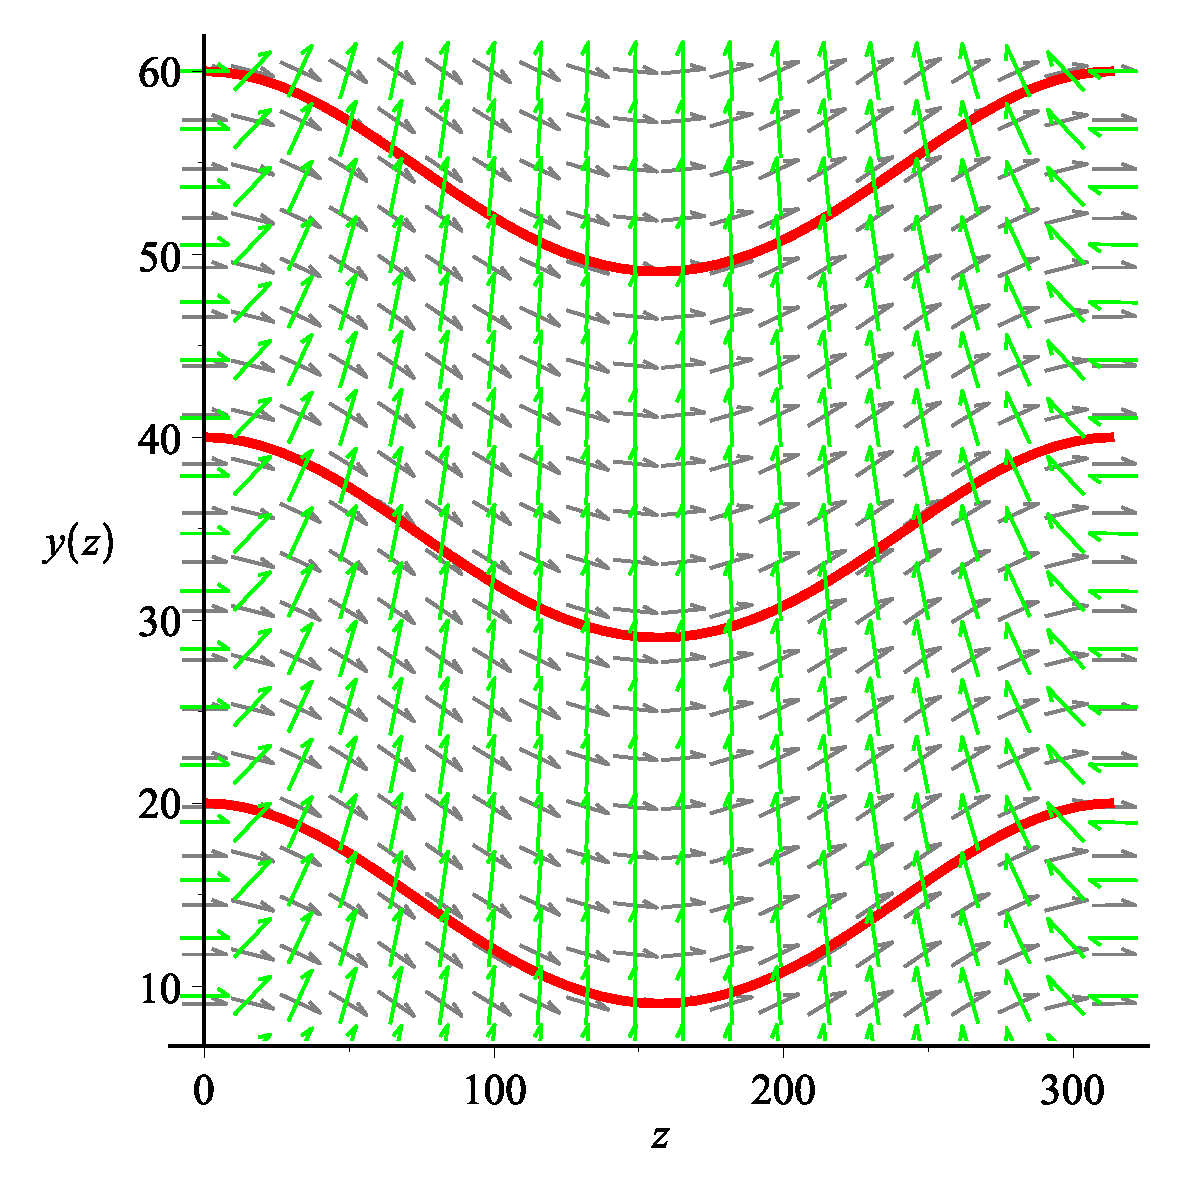
\includegraphics[scale=0.2]{Visualization4}
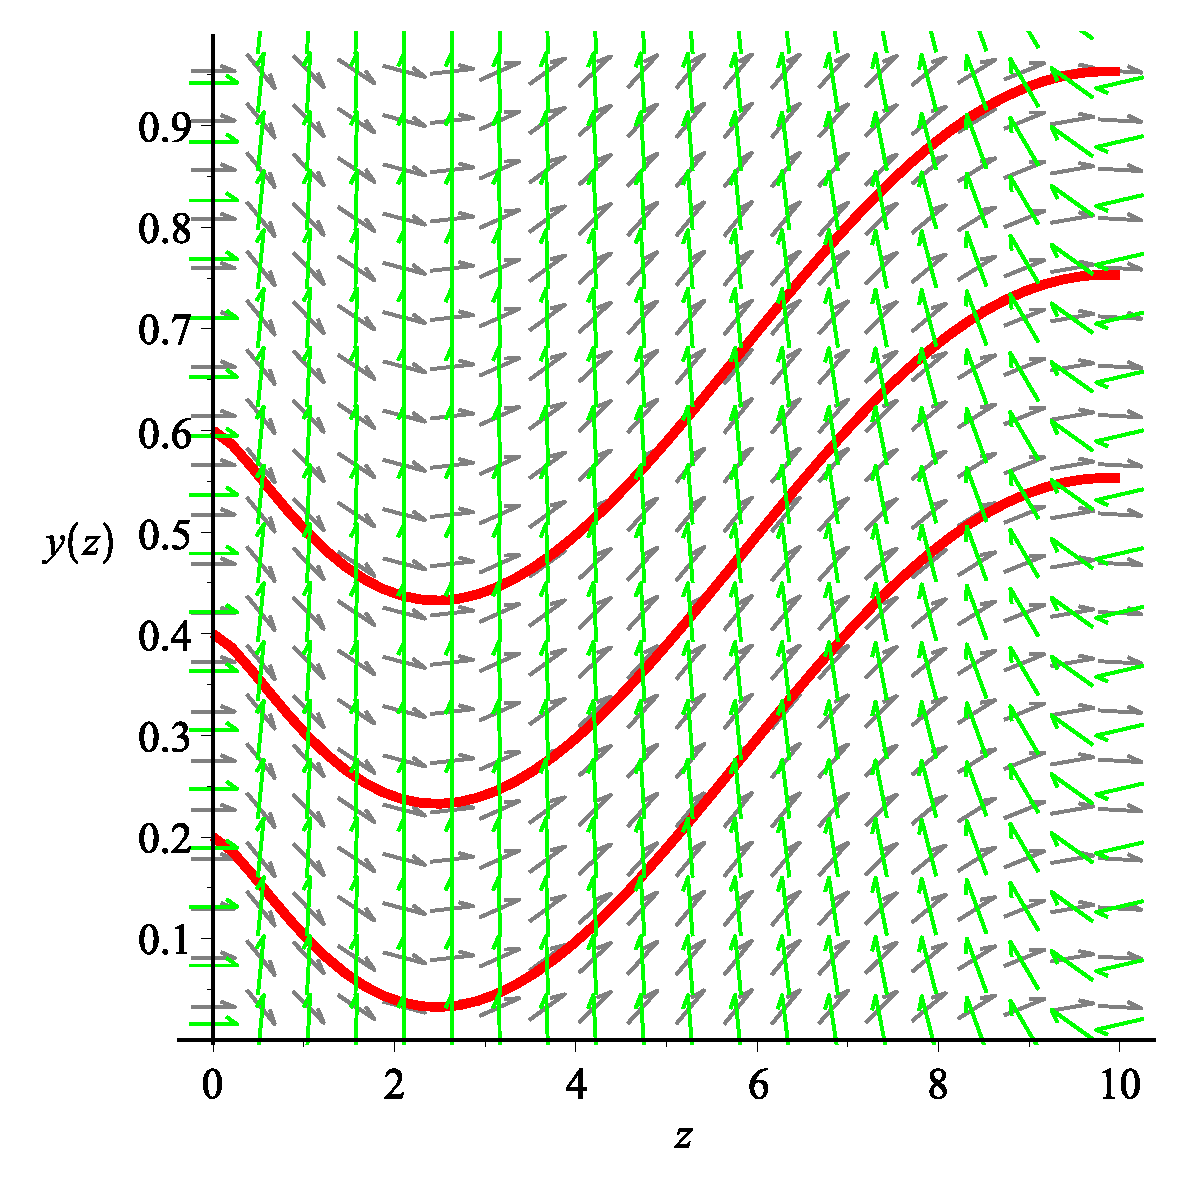
\includegraphics[scale=0.2]{Visualization3}
\caption{Ray tracing in anisotropic media with variable optical axes, $\theta=z$ (left) and $\theta=sqrt{z}$ (right),  the  green arrows  indicate orientations of the third principle axis and the red lines  indicate ray trajectories  in the media.}
\label{curvedspace2}
\end{figure}

As we can see in the Fig. \ref{curvedspace2}, the light geodesics through these media
 are not straight lines and moreover, it seems that these surface are under tensions.  Therefore,  we expect a non-zero Riemann tensor for the corresponding metric.  
we can construct the  metric of  this two dimensional distorted surface, Fig \ref{curvedspace2},  by choosing two bases of this space as:
\begin{eqnarray}\label{base}
e_{1}=c_{1}
\begin{pmatrix}
1\\0
\end{pmatrix} \qquad
e_{2}=c_{2}
\begin{pmatrix}
0\\1
\end{pmatrix}
\end{eqnarray}

 where coefficients $c_{1}$ and $c_{2}$  are scalar functions which provides sufficient conditions for null geodesics  $\mathrm{d}s^{2}=0$ . Using these bases (\ref{base}), the metric components \cite{leonhardt2012geometry} are  given by:
 
\begin{eqnarray}
&g_{ij}=e_{i}\cdot e_{j}.
\end{eqnarray}

Therefore, we can write the space-time metric in matrix form as,   
\begin{equation}
\mathbf{g}=
\begin{pmatrix}
-1&0&0\\
0&c_{1}&0\\
0&0&c_{2}
\end{pmatrix}
\end{equation}
or equivalently in the form of Riemann line element as
\begin{eqnarray}
\mathrm{d}s^{2}=-c^{2}dt^{2}+c_{1}^{2} dy^{2} +c_{2}^{2} dz^{2}
\end{eqnarray}
The null geodesics condition,$\mathrm{d}s^{2}=0$,  results,
\begin{eqnarray}
 c_{1}^{2} dy^{2} +c_{2}^{2} dz^{2}-c^{2}dt^{2}=0
\end{eqnarray}
We can assume $c_{1}=c_{2}$, so we achieve
\begin{eqnarray}\label{c1c2}
c_{1}^{2}=c_{2}^{2} =\dfrac{c^{2}dt^{2}}{dl^{2}}
\end{eqnarray}
where $dl^{2}=dy^{2}+dz^{2}$.

On the other hand, The surface of equal phases for the propagating light fields define as the solutions of:

\begin{equation}\label{level}
\mathrm{d}{\varphi(r,t)}=0.
\end{equation}

This condition (\ref{level}) results in 

\begin{equation}\label{phase1}
\mathbf{k}\cdot {\mathrm{d}\mathbf{r}}-\omega\mathrm{d}{t}=0.
\end{equation}
our equivalently 
\begin{equation}
c dt=n\hat{U}\cdot {\mathrm{d}\mathbf{r}}
\end{equation}.

Using equation (\ref{imp-d}) and (\ref{extra.d}) we can write the following relation:


\begin{eqnarray}\label{cdt}
c dt=\dfrac{\varepsilon_{2} \sin^{2}{\theta} + \varepsilon_{3}\cos^{2}{\theta}}{\sqrt{\varepsilon_{2}^{2} \sin^{2}{\theta} + \varepsilon_{3}^{2}\cos^{2}{\theta}}}dl
\end{eqnarray}
Substituting (\ref{cdt}) in relation (\ref{c1c2}) the coefficient $c_{1}$ and $c_{2}$ are easily determined,
\begin{eqnarray}
c_{1}^{2}=c_{2}^{2}=n\dfrac{\left(\varepsilon_{2} \sin^{2}{\theta} + \varepsilon_{3}\cos^{2}{\theta}\right)^{2}}{\varepsilon_{2}^{2} \sin^{2}{\theta} + \varepsilon_{3}^{2}\cos^{2}{\theta}}
\end{eqnarray}

\begin{eqnarray}
\mathrm{d}s^{2}=-c^{2}dt^{2}+ n\dfrac{\left(\varepsilon_{2} \sin^{2}{\theta} + \varepsilon_{3}\cos^{2}{\theta}\right)^{2}}{\varepsilon_{2}^{2} \sin^{2}{\theta} + \varepsilon_{3}^{2}\cos^{2}{\theta}}dl^{2}
\end{eqnarray}

According to the previous section the refractive index of the extraordinary ray is differ from the refractive index of the light in the impedance-matched media. Therefore, despite the  same trajectory of the ray in these media the space time metrics of them is different. The electric media construct the following metric for the extraordinary ray

\begin{eqnarray}
ds^{2}=- c^{2}dt^{2} + \dfrac{\varepsilon_{2}\varepsilon_{3}\left({\varepsilon_{2} \sin^{2}{\theta} + \varepsilon_{3}\cos^{2}}\right)}{\left({\varepsilon_{2}^{2} \sin^{2}{\theta} + \varepsilon_{3}^{2}\cos^{2}}\right)} {(dy^{2}+dz^{2})}.
\end{eqnarray}
whereas the impedance matched media appear as following metric for the light ray

\begin{equation}\label{metric-im}
ds^{2}=- c^{2}dt^{2} + \dfrac{\varepsilon_{1}\varepsilon_{2}\varepsilon_{3}\left({\varepsilon_{2} \sin^{2}{\theta} + \varepsilon_{3}\cos^{2}}\right)}{\left({\varepsilon_{2}^{2} \sin^{2}{\theta} + \varepsilon_{3}^{2}\cos^{2}}\right)} {(dy^{2}+dz^{2})}.
\end{equation}

On the other hand, using  transformation optics \cite{leonhardt2012geometry},  we can find the space metric for impedance-matched media by 

\begin{equation}
\mathbf{g}=(\det{ \boldsymbol{\varepsilon}})\boldsymbol{\varepsilon}^{-1}.
\end{equation}
This metric, for the case in Fig. \ref{figure1}, can be written in the form 

\begin{align}\label{t-metric}
&\mathbf{g}_{imp}(y-z)= \nonumber\\
&\begin{pmatrix}
\varepsilon_{1}(\varepsilon_{2} \sin^{2}{\theta} +\varepsilon_{3}\cos^{2}{\theta})& \varepsilon_{1}(\varepsilon_{2}-\varepsilon_{3})\sin{\theta} \cos{\theta}\\
\varepsilon_{1}(\varepsilon_{2}-\varepsilon_{3})\sin{\theta} \cos{\theta}&\varepsilon_{1}(\varepsilon_{2} \cos^2{\theta} +\varepsilon_{3}\sin^{2}{\theta})
\end{pmatrix}.
\end{align}

At first glance, the metric (\ref{t-metric}) is different from the metric (\ref{metric-im}), but , by using following relation:  

\begin{equation}\label{dz}
\begin{split}
\varepsilon_{2} \varepsilon_{3}&=(\varepsilon_{2} \cos^2{\theta} +\varepsilon_{3}\sin^{2}{\theta})(\varepsilon_{2} \sin^{2}{\theta} +\varepsilon_{3}\cos^{2}{\theta})  \\
&   \qquad  -\left[ (\varepsilon_{2}-\varepsilon_{3})\sin{\theta} \cos{\theta}\right]^{2},
\end{split}
\end{equation}

 we obtain that the metrics (\ref{metric-im})  and (\ref{t-metric}) are equivalent.
 this can be considered as a verification of our method.
 
Also, Using differential geometry relations, we can investigate the curvature of the above conformal flat spaces. 
 Riemann curvature tensor given by \cite{leonhardt2012geometry}
\begin{equation}\label{Riemann}
R^{i}_{jkl}\equiv \Gamma^{i}_{jl,k}-\Gamma^{i}_{jk,l}+\Gamma^{i}_{mk}\Gamma^{m}_{jl}-\Gamma^{i}_{ml}\Gamma^{m}_{jk}
\end{equation}

where $\Gamma^{i}_{jk}$ is Christoffel symbol and the comma notation "$,$" refers to partial differentiation.  The Christoffel symbol can be expressed in terms of the metric component as
\begin{equation}\label{cr}
\Gamma^{i}_{jk}=\dfrac{1}{2} g^{il}(g_{lj,k}+g_{lk,j}-g_{jk,l})
\end{equation}

For the metric (\ref{m2}), which is conformally two dimensional flat spaces, $g_{ij}=n^{2}\delta_{ij}$,  we can obtain Christoffel symbol  from relation

\begin{equation}\label{cr1}
\Gamma^{i}_{ij}=\dfrac{1}{2n^{2}}n^{2}_{,j}.
\end{equation}
Using this relation, (\ref{cr1}), Riemann curvature tensor, (\ref{Riemann}) can be achieved as 
\begin{equation}
\begin{split}
&R_{11}=R_{22}=\\
&\dfrac{1}{2n^{4}} \lbrace (\dfrac{\partial}{\partial z}n^{2})^{2} +(\dfrac{\partial}{\partial y}n^{2})^{2}\rbrace -\dfrac{1}{2n^{2}}\lbrace(\dfrac{\partial}{\partial z}\dfrac{\partial}{\partial z}n^{2})+(\dfrac{\partial}{\partial y}\dfrac{\partial}{\partial y}n^{2})\rbrace
\end{split}
\end{equation}
We calculated this tensor for the above example of the variable axes media, $\theta=z$ and find that 
 \begin{equation}
R_{ii}\neq 0.
\end{equation}

Consequently, the medium with $\theta=z$ have a non-zero Riemann curvature tensor and appears as a curved space for the extraordinary light. Therefore, we can use variable optical axes media for realizing curved space time in the laboratory. 

\section{Conclusion}\label{conclusion}

In this paper we extend the method of transfer matrix to study the optical properties of a very especial optical medium. The media is an engineered inhomogeneous material: The stratified, homogenous layers with varying optical axes.  We show that this uncommon form of inhomogeneity would  also results in the emergence of effective geometry in the medium. Our finding results in a new method for manipulation of electromagnetic waves. 
 


\section*{Acknowledgment}
S.A.M, R.R wish to thank the office of graduate studies of the university of Isfahan for their support.

\bibliography{mybib}

\end{document}

